\subsection{Lavpasfilter}
For at teste om lavpasfilteret fungerer efter kravene stillet i \autoref{sec:lavpas_krav} visualiseres forskellen mellem det ufiltrede signal og det filtrede signal. Signalerne der sendes ind er fra det optagede signal fra pilotforsøget \autoref{sec:pilotforsoeg}. Disse sendes til mikrokontrollen via UART-forbindelse, hvorved der modtages den retunerede værdi. De sendte og returnerede værdier er visualiseret i MATLAB og fremgår af \autoref{fig:lavpas_imp}

\begin{figure}[H]
\centering
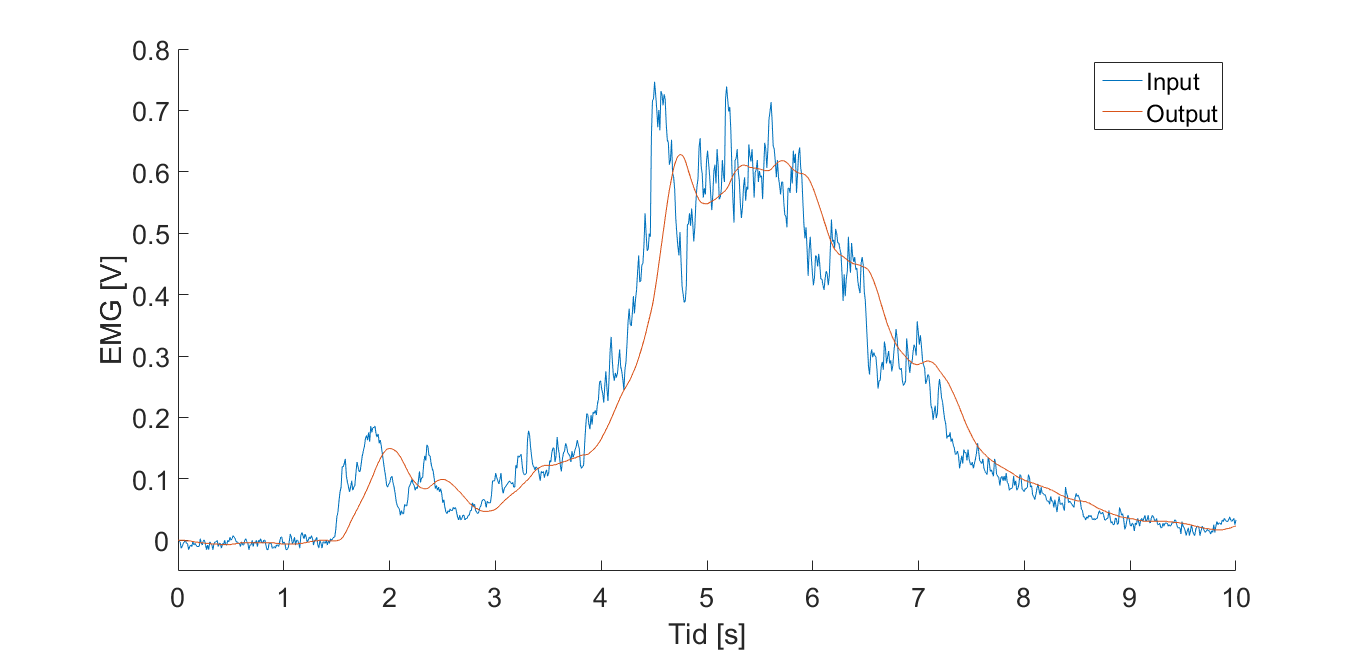
\includegraphics[width=0.8\textwidth]{figures/EMG_test}
\caption{Lavpasfilter programmeret i PSoC visualiseret i MATLAB}
\label{fig:lavpas_imp}
\end{figure}

På baggrund af disse resultater fremgår at de ønskede krav om maksimal fladhed samt undgå ripples ved brug af Butterworth lavpasfilter er overholdt. 
Deruodver fremgår det at inputsignalet følger det ufiltrede signal dog med et delay. Til måling af behandlingstiden af dette, programmeres en timer funktion i mikrokontrolleren, der retunerer behandlingstiden til MATLAB. Ud fra dette ses et delay på 39 sekunder og 56 milisekunder.


For at vurdere om filteret dæmper i forhold til de opstillede krav, udføres en sweep-test af frekvenser fra $0-15~Hz$ med en funktionsgenerator. Dette frekvensområde er valgt på baggrund af målinger fra \autoref{sec:pilotforsoeg}, hvor det fremgår at signalet ligger mellem $0,4-10Hz$.  Da funktionsgeneratoren ikke kan indstilles til en frekvens på $0~Hz$ indstilles denne til $1 \mu~Hz$. Amplituden sættes til $1~Vpp$. Resultatet af denne test fremgår af \autoref{fig:lavpas_sweep}. 


\begin{figure}[H]
\centering
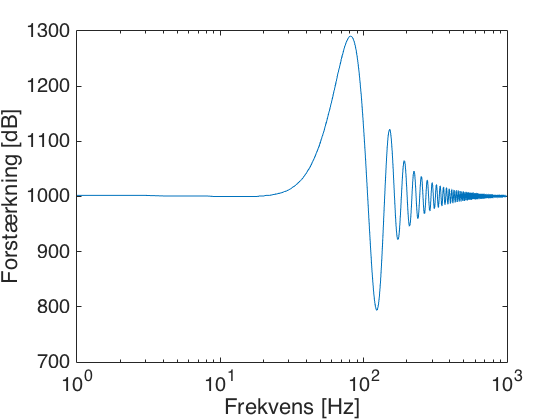
\includegraphics[width=0.8\textwidth]{figures/bodeplot_lavpas}
\caption{Bodeplot fra sweep-test af et filterede signal sinus signal med en frekvens på $1\mu~Hz$ til $15~Hz$.}
\label{fig:lavps_sweep}
\end{figure}

På baggrund af disse resultater fremgår at de ønskede krav om en knækfrevens på ...

